%% what_is_compgen.tex
%% Author: Leighton Pritchard
%% Copyright: James Hutton Institute
%% Introductory slides: What is Comparative Genomics?





%
\begin{frame}
  \frametitle{What Is Comparative Genomics?}
  \Large{
    \textcolor{olive}{
      \textbf{
      The combination of genomic data, and comparative and evolutionary biology, to address questions of   genome structure, evolution, and function.
      }
    }
  }
\end{frame}

%
\begin{frame}
  \frametitle{Evolution is the central concept}
  \begin{center}
    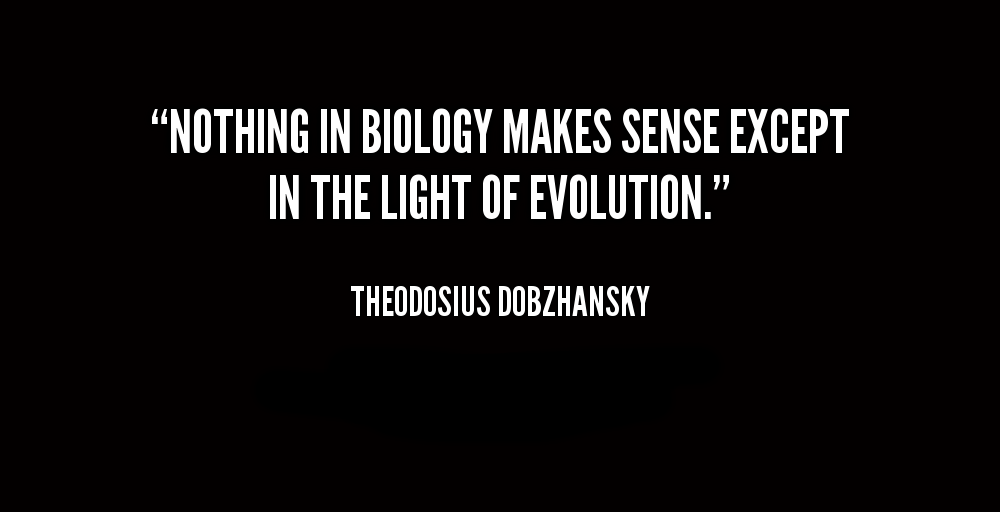
\includegraphics[width=\textwidth]{images/dobzhansky_quote}
  \end{center}  
\end{frame}

%
\begin{frame}
  \frametitle{Comparison of physical features}
  How do we determine that features share a common ancestor? \\
  \begin{center}
    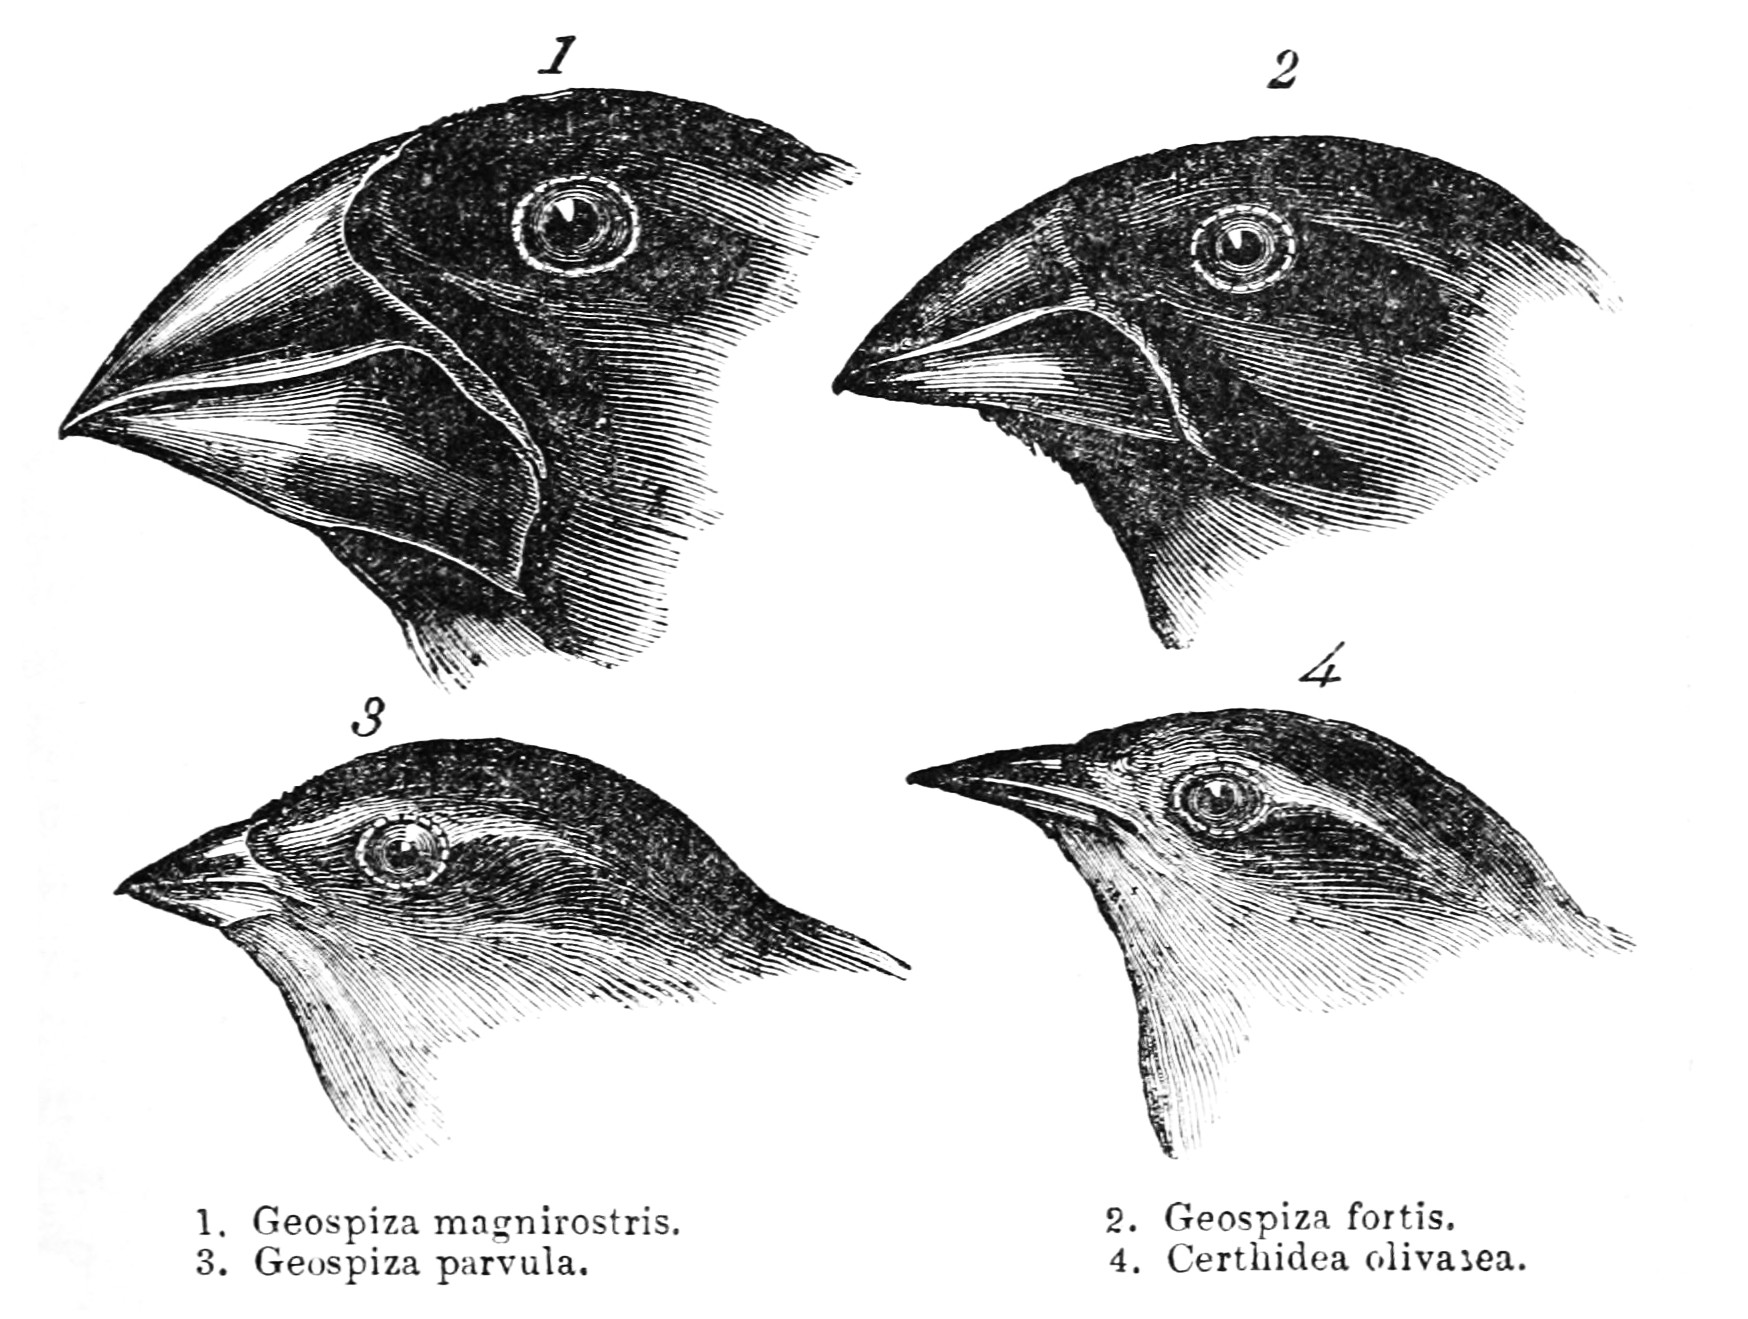
\includegraphics[width=0.8\textwidth]{images/darwin_finches}
  \end{center}  
\end{frame}

%
\begin{frame}
  \frametitle{Comparison of sequence features}
  How do we determine that features share a common ancestor? \\
  \textcolor{hutton_blue}{Multiple sequence alignment of ATP synthase} \\
  \begin{center}
    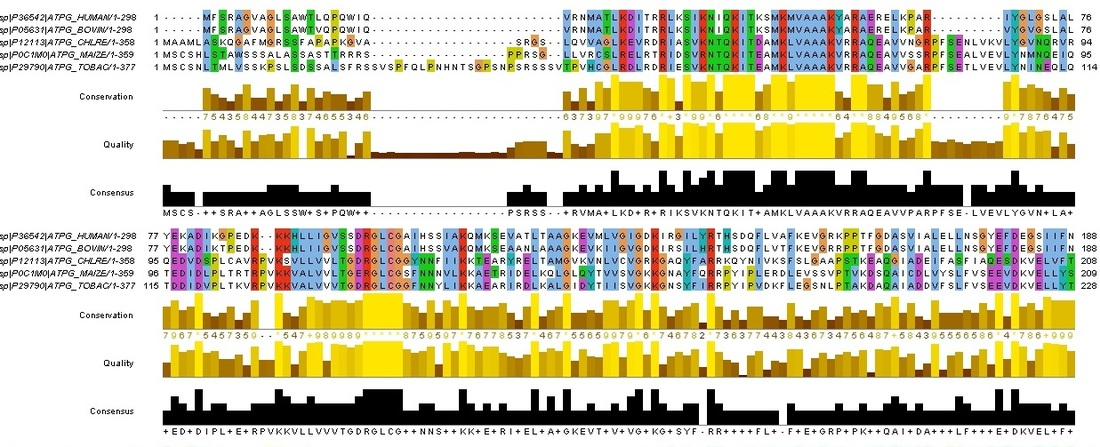
\includegraphics[width=\textwidth]{images/atp_synthase_alignment}
  \end{center}  
\end{frame}

%
\begin{frame}
  \frametitle{Comparison of genome features}
  How do we determine that features share a common ancestor? \\
  \textcolor{hutton_blue}{Similarity of individual features (feature sequence)} \\
  \begin{center}
    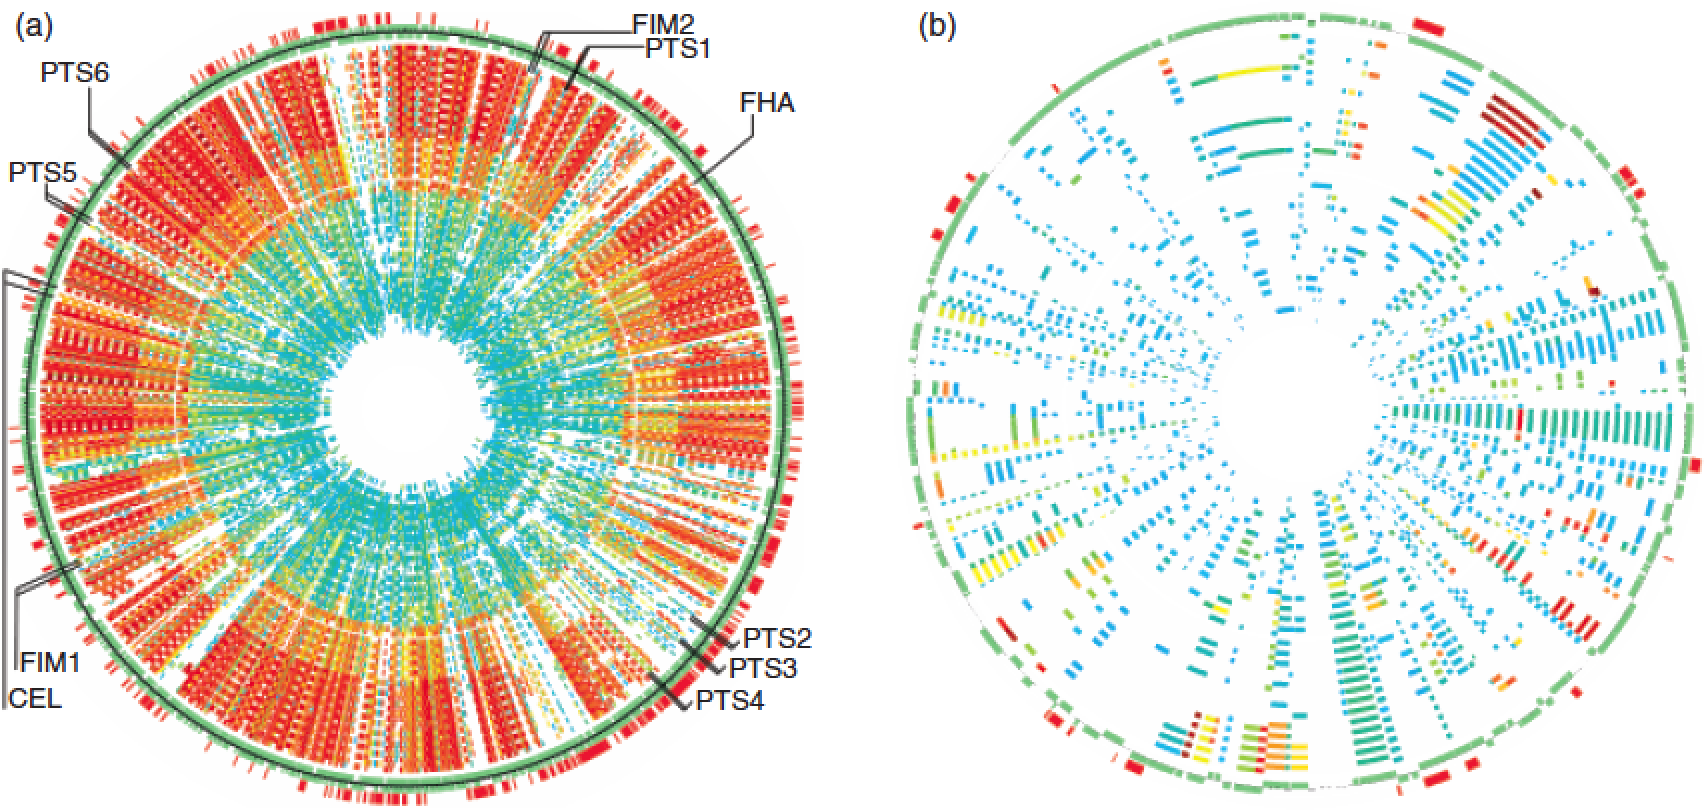
\includegraphics[width=\textwidth]{images/salmonella_circular_comparison}
  \end{center}  
\end{frame}

%
\begin{frame}
  \frametitle{Comparison of genome features}
  How do we determine that features share a common ancestor? \\
  \textcolor{hutton_blue}{Similarity of individual features (ordering and arrangement)} \\
  \begin{center}
    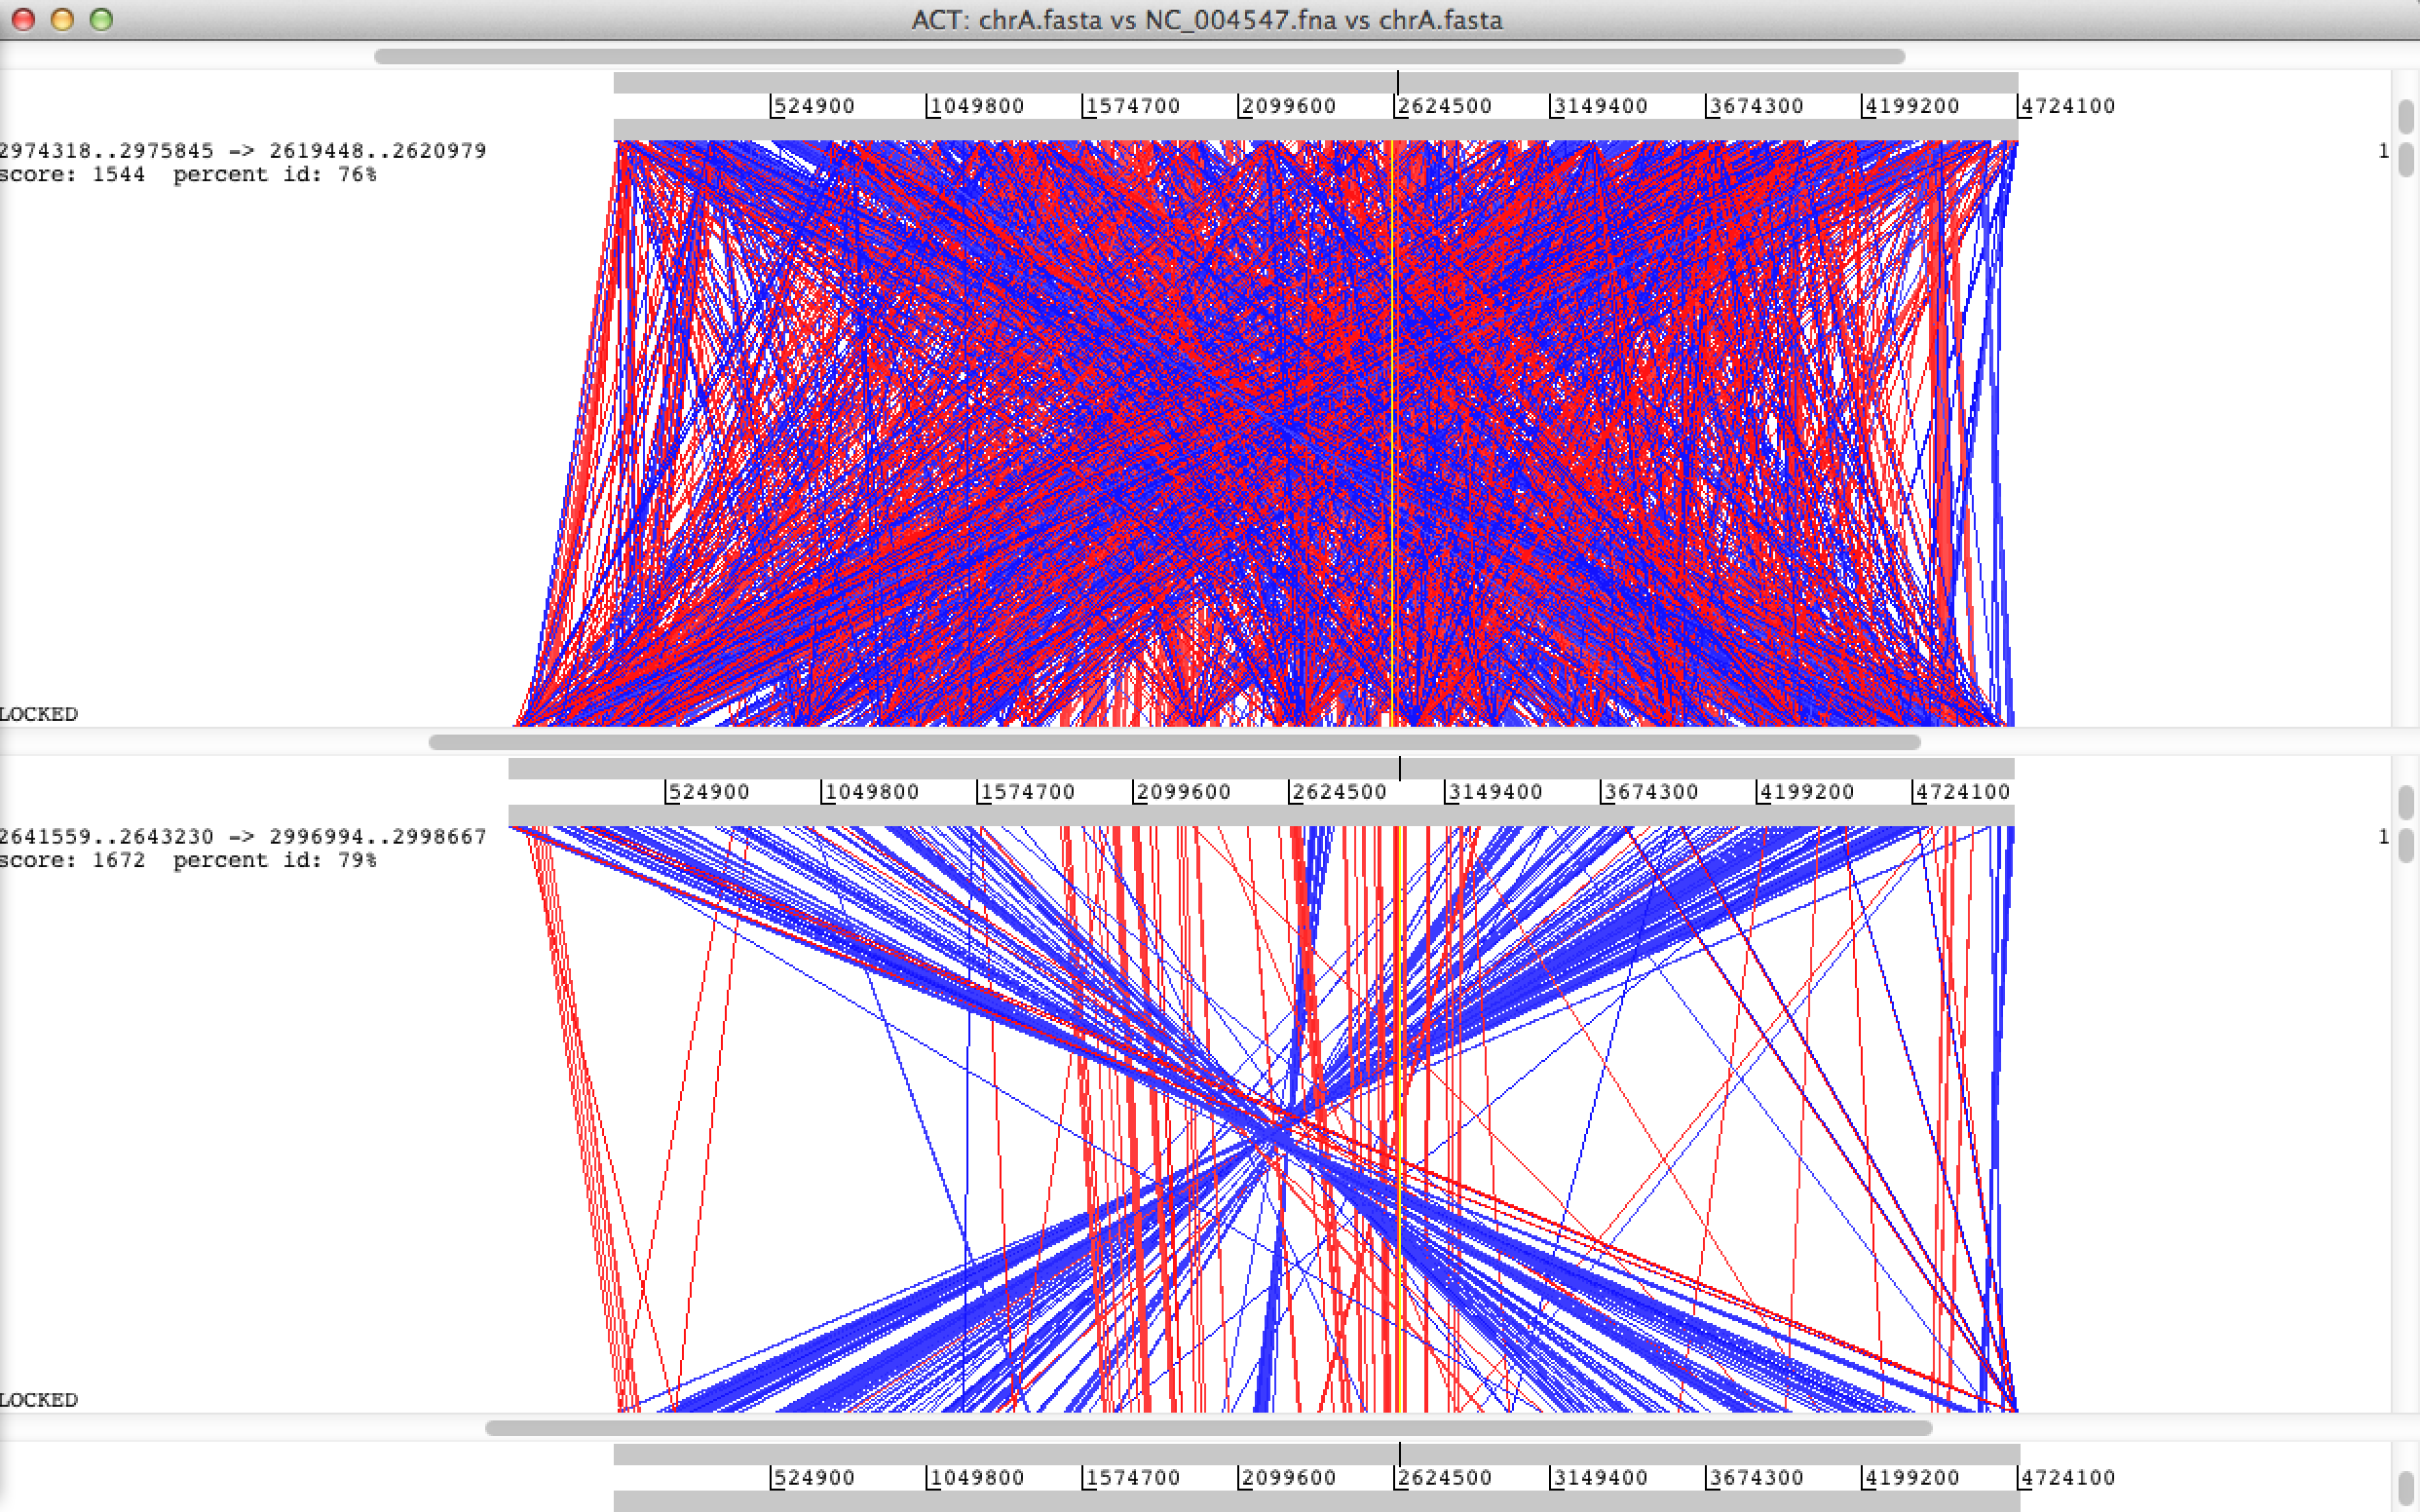
\includegraphics[width=0.8\textwidth]{images/act_rearrangement}
  \end{center}  
\end{frame}

%
\begin{frame}
  \frametitle{Why comparative genomics?}
    \begin{columns}[c] 
      \column{.6\textwidth} 
        \begin{itemize}
         \item \textcolor{hutton_green}{Genome features are heritable characteristics}
         \item \textcolor{hutton_purple}{Related organisms share ancestral genomes}
         \item \textcolor{hutton_blue}{Related organisms inherit common genome features}
         \item \textcolor{RawSienna}{Genome similarity $\propto$ relatedness? (phylogenomics)}
        \end{itemize}
      \column{.4\textwidth}
        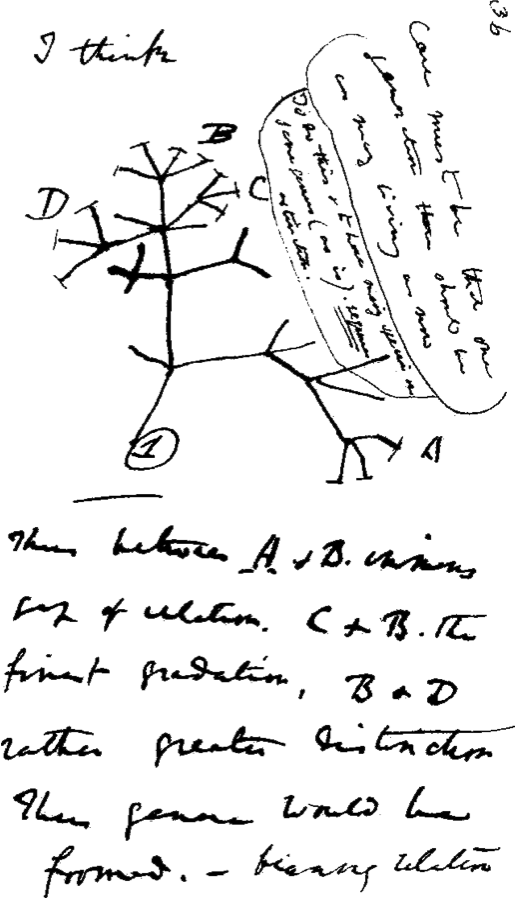
\includegraphics[width=\textwidth]{images/darwin_tree}
    \end{columns}  
\end{frame}

%
\begin{frame}
  \frametitle{Why comparative genomics?}
    \begin{columns}[c] 
      \column{.6\textwidth} 
        \begin{itemize}
         \item \textcolor{hutton_green}{Genomes carry functional elements under selection pressure}
         \item \textcolor{hutton_blue}{Deleterious functional elements are lost through selection}         
         \item \textcolor{hutton_purple}{Organisms with similar phenotype carry similar functional elements}
         \item \textcolor{RawSienna}{Genome similarity $\propto$ phenotype? (functional genomics)}         
        \end{itemize}
      \column{.4\textwidth}
        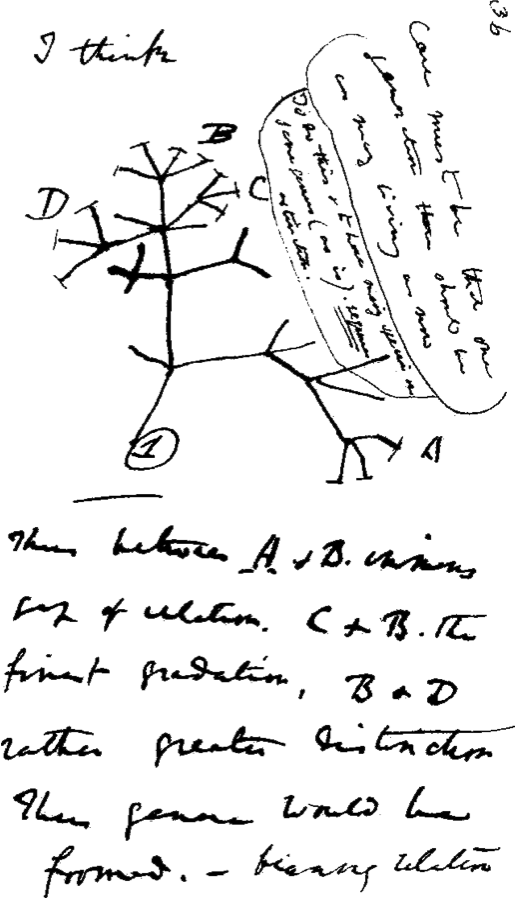
\includegraphics[width=\textwidth]{images/darwin_tree}
    \end{columns}  
\end{frame}

%
\begin{frame}
  \frametitle{Why comparative genomics?}
    \begin{columns}[c] 
      \column{.6\textwidth} 
        \begin{itemize}
         \item \textcolor{hutton_purple}{Functionally-optimised elements are conserved}
         \item \textcolor{hutton_blue}{(Functional elements can be transferred non-heritably)}   
         \item \textcolor{RawSienna}{Genome feature similarity $\implies$ common function? (genome annotation)}
         \item \textcolor{red}{Transfer functional information from model systems (\textit{E. coli}, \textit{A. thaliana}, \textit{D. melanogaster}) to non-model systems}
        \end{itemize}
      \column{.4\textwidth}
        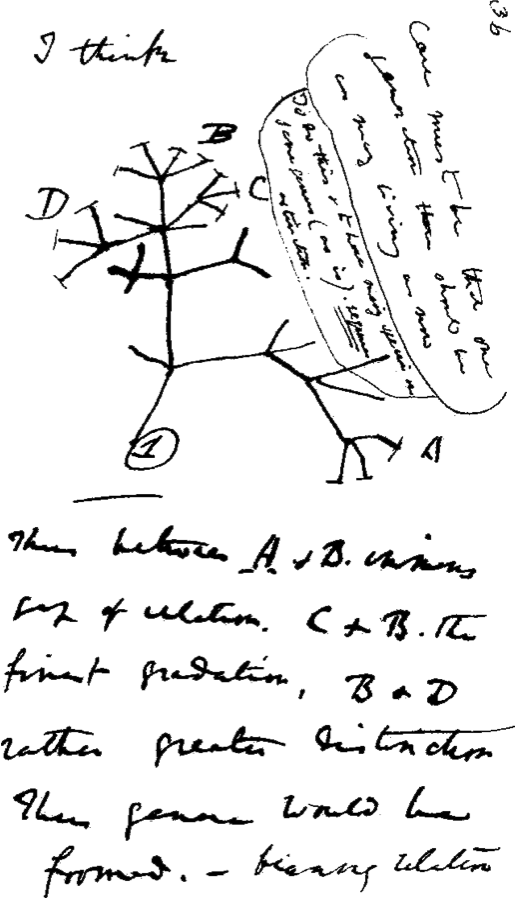
\includegraphics[width=\textwidth]{images/darwin_tree}
    \end{columns}  
\end{frame}


